% SOICT 2026 submission — Springer CCIS format (single-blind: keep author names).
% Requires the Springer LNCS/CCIS class `llncs.cls` + `splncs04.bst` from
% https://soict.org/wp-content/uploads/2025/09/Latex-Template-for-Springer.zip
% Max 12 pages excluding references. Figure: convert docs/paper/diagrams/soict_harlstmgat.svg -> PDF.
\documentclass[runningheads]{llncs}
\usepackage{graphicx}
\graphicspath{{diagrams/}}   % figure lives in docs/paper/diagrams/ (do NOT add ./ — collides with output pdf)
\usepackage{booktabs}
\usepackage{amsmath}
\usepackage[T1]{fontenc}

\begin{document}

\title{Multi-Horizon Stock Volatility Forecasting}

\author{Author One\inst{1} \and Author Two\inst{1}}
\authorrunning{Multi-Horizon Volatility Forecasting}
\institute{Affiliation, City, Country \\ \email{\{author1,author2\}@example.edu}}

\maketitle

\begin{abstract}
We evaluate whether a deep sequence model or a cross-sectional graph-attention branch changes multi-horizon
daily Parkinson-variance forecasts relative to a linear Heterogeneous Autoregressive model, extended to five features (HAR-X), on the
Vietnamese equity market --- VN30 and VN100 --- under panel-correct inference.
Three models share the same five node features: a linear HAR-X, a
five-feature LSTM, and a five-feature LSTM+GAT (directed volume$\to$Parkinson Top-5 weighted two-hop
attention). We report five metrics (MSE, RMSE, MAE, QLIKE, $R^2$) with equal weight and assess significance
with the date-clustered Diebold--Mariano (DM) test; predictions are floored at $10^{-2}$ times the per-node
training mean. The primary target is short-term (horizons $h\in\{1,5\}$); $h\in\{10,22\}$ are an extended
study. HAR-X has the lowest QLIKE at every horizon except VN100 $h1$ (where the LSTM+GAT point estimate is
marginally lower, not significantly), and no learned model has a significantly
lower QLIKE than HAR-X at any horizon (date-clustered DM, $p\ge0.05$). At $h1$ and $h5$ the deep models have the lowest MAE on
VN100 (LSTM vs HAR-X, $p<0.001$), and the LSTM+GAT has a significantly lower QLIKE than the no-graph LSTM in
both panels (VN100 $h1$ $p<0.001$, $h5$ $p=0.022$; VN30 $h1$ $p<0.001$, $h5$ $p=0.031$), equal to HAR-X's QLIKE
level at VN100 $h5$ (0.5690 vs 0.5633). At $h10$ and $h22$ HAR-X has the lowest MSE, RMSE, QLIKE and $R^2$, and
the LSTM+GAT-vs-LSTM QLIKE difference is not significant ($p\ge0.55$). The ranking is metric- and
horizon-dependent, so all five metrics are reported with equal weight. Methodologically, a naive
per-observation DM test on this cross-sectionally dependent panel overstates significance by roughly the square root of the number of stocks.
As an out-of-sample extension we apply the same configuration and protocol, without any retuning, to the broader
Vietnamese universe (the HOSE and HNX exchanges, 352 and 154 tickers): on the less-liquid HNX panel the deep and
graph models attain a significantly lower QLIKE than HAR-X at $h1$, $h10$ and $h22$ and the LSTM+GAT a
significantly lower QLIKE than the no-graph LSTM at $h10$ and $h22$, whereas on the more-liquid HOSE panel no
learned model differs significantly from HAR-X on QLIKE.
\keywords{Volatility forecasting \and HAR \and LSTM \and Graph Attention Network \and Diebold--Mariano.}
\end{abstract}

\section{Introduction}
Daily volatility forecasting underpins risk management, position sizing and derivative pricing. The HAR model
of Corsi~\cite{corsi2009} is a linear benchmark: a few OLS coefficients on daily, weekly and monthly
aggregates of realized volatility capture much of the long-memory structure. Deep sequence models and graph
neural networks are frequently proposed to capture nonlinear temporal dynamics and cross-sectional spillovers,
and the evidence that they beat HAR out of sample is mixed; positive claims are often confounded by
data-design choices, such as a common-date intersection that discards most of the panel or a naive
significance test on cross-sectionally dependent data.

This paper measures, under a single panel-correct evaluation on the Vietnamese equity market, whether the
temporal nonlinearity or the cross-sectional graph changes the forecast relative to a linear HAR-X. We ask: (1)
Does a deep temporal LSTM over the shared feature set change the out-of-sample forecast relative to the linear
HAR-X, and at which horizons and metrics? (2) Does a cross-sectional Graph Attention Network branch --- here a
directed volume$\to$Parkinson weighted graph --- change the forecast relative to the same-feature no-graph
LSTM? To answer these we use a \emph{masked panel}: rather than intersecting to the dates on
which every ticker is present, we keep the union of trading dates with node and target masks for tickers not
yet listed on a given date, so late-listed tickers are included without dropping whole dates and every model
--- including the graph model --- is trained and evaluated on the same panel with the same five features.

Our contributions are: (i) a multi-horizon benchmark on the masked VN30/VN100 panel that holds
the feature set and the data design fixed across HAR-X, an LSTM and an LSTM+GAT, so any difference is
attributable to a single component; (ii) per-horizon results on all five metrics with the date-clustered DM
test --- HAR-X has the lowest QLIKE at every horizon except VN100 $h1$ (not significantly), with no learned model significantly lower at any horizon, the deep models
have the lowest short-horizon MAE on VN100, and the LSTM+GAT has a significantly lower QLIKE than the no-graph
LSTM at $h1$ and $h5$ in both panels but not at $h10$ or $h22$; and (iii) a methodological contribution --- the
date-clustered DM test, since a naive per-observation test overstates significance by roughly the square root of the number of stocks. Every number is taken from a stored results file.
We additionally report an out-of-sample extension to the broader Vietnamese universe (the HOSE and HNX
exchanges): applied without retuning, the deep and graph models are competitive-to-better on the less-liquid
HNX exchange and show no significant QLIKE difference from HAR-X on the more-liquid HOSE exchange.

\section{Related Work}
\textbf{HAR and classical models.} HAR~\cite{corsi2009} approximates the long memory of realized volatility
with a daily/weekly/monthly cascade; recent work reports that rolling-window and specification choices, rather
than model class, often account for measured differences from HAR~\cite{audrino2025}. HARQ~\cite{harq2016}
exploits measurement error, and GARCH-family models remain standard conditional-variance benchmarks. We use
HAR-X as the linear baseline and GARCH(1,1) as a classical benchmark. \textbf{Deep and graph models.} LSTMs~\cite{lstm1997} are widely applied to
financial series, and graph neural networks model cross-asset spillovers, e.g.\ Graph Attention
Networks~\cite{gat2018}, multivariate realized-volatility GNNs~\cite{chen2022} and spillover-aware GNN-HAR
hybrids~\cite{gnnhar2025}; reported effects vary across studies and data designs. Volatility spillover
measurement has a long econometric tradition~\cite{dy2012}. \textbf{Graph construction.} Our graph uses a
directed volume$\to$Parkinson relation (each node attends to its Top-5 volume-shock leaders, edge-weighted,
over two hops), motivated by volume leading volatility. \textbf{Evaluation.} Volatility is latent, so we use
the proxy-robust QLIKE loss~\cite{patton2011} alongside MSE, with significance by the Diebold--Mariano
test~\cite{dm1995} and the Harvey--Leybourne--Newbold small-sample correction~\cite{hln1997}.

\section{Method}
\textbf{Target and features.} The target is the Parkinson variance~\cite{parkinson1980} at day $t{+}h$, a
non-negative point forecast. The primary target is short-term, horizons $h\in\{1,5\}$ (one trading day and one
trading week ahead); $h\in\{10,22\}$ (two weeks and roughly one trading month) are an extended study. All
three feature-based models (HAR-X, LSTM, LSTM+GAT) use the same five node features per ticker at $t$: the daily Parkinson variance, its 5-day
rolling mean (weekly), its 22-day rolling mean (monthly), a market Parkinson factor (the causal cross-sectional
median of the square-root Parkinson variance) and a 20-day volume z-score.

\textbf{Models.} \emph{HAR-X} (baseline): pooled OLS on the five features (the HAR cascade augmented with a market Parkinson factor and a volume z-score), linear. \emph{LSTM}: a two-layer LSTM
(hidden 64) over the lookback window of the five features; a single pooled model is trained over all tickers,
each standardized by its own scaler fit on training rows only, with a linear output inverse-transformed for
evaluation (dropout, weight decay, gradient clipping, ReduceLROnPlateau, early stopping). \emph{LSTM+GAT}
(Fig.~\ref{fig:arch}): the LSTM branch plus a Graph Attention Network branch~\cite{gat2018} that reads the five
node features at $t$ and attends over a directed volume$\to$Parkinson Top-5, edge-weighted, two-hop graph
estimated on training rows only; the branches are concatenated into an MLP head. The leave-one-out comparison
against the same-feature LSTM isolates the graph's marginal contribution. \emph{GARCH}: a GARCH(1,1)
conditional-variance model fit per ticker on the training Parkinson-variance series (via pseudo-returns), with
persistence capped at $0.999$ by variance targeting so near-integrated fits do not diverge over the frozen
multi-step forecast path; a classical benchmark that forecasts the variance series directly and does not use
the node features.

\textbf{Masked panel.} A GAT operates over a common-date cross-section, which naively forces a
common-date intersection (only dates on which every ticker is present) that discards most ticker-days and
places the whole test set in one recent period. We instead use a masked panel: the GAT operates
over a common-date cross-section with node and target masks for tickers not yet listed on a given date, so
late-listed tickers are included without dropping whole dates, and a mask-aware loss ignores absent tickers.
Every model is trained and evaluated on the same panel with the same five features and split (VN100: 46{,}308
masked obs over 454 test dates at $h1$; VN30: 10{,}106 obs over 326 test dates at $h1$).

\textbf{Protocol.} Each configuration runs five seeds, up to 20 epochs with early stopping. We report MSE,
RMSE, MAE, QLIKE and $R^2$, seed-averaged, with equal weight; predictions are floored at $10^{-2}$ times the
per-node training mean, applied identically to every model. Significance uses the \emph{date-clustered}
Diebold--Mariano test: the per-observation loss differential is collapsed to one value per calendar date
before the statistic (HLN correction, HAC lag $h{-}1$) is computed. This is the panel-correct treatment for a
cross-section that shares each trading date; a naive per-observation test treats the effective sample as the
number of tickers times the number of dates and inflates the statistic by roughly the square root of the number of stocks (about
six on VN30, ten on VN100). We report two targeted contrasts --- LSTM vs HAR-X and LSTM+GAT vs LSTM --- on QLIKE
and MAE.

\begin{figure}[t]
\centering
% figure generated by docs/paper/diagrams/generate_arch.py -> diagrams/soict_harlstmgat.{pdf,png,svg}
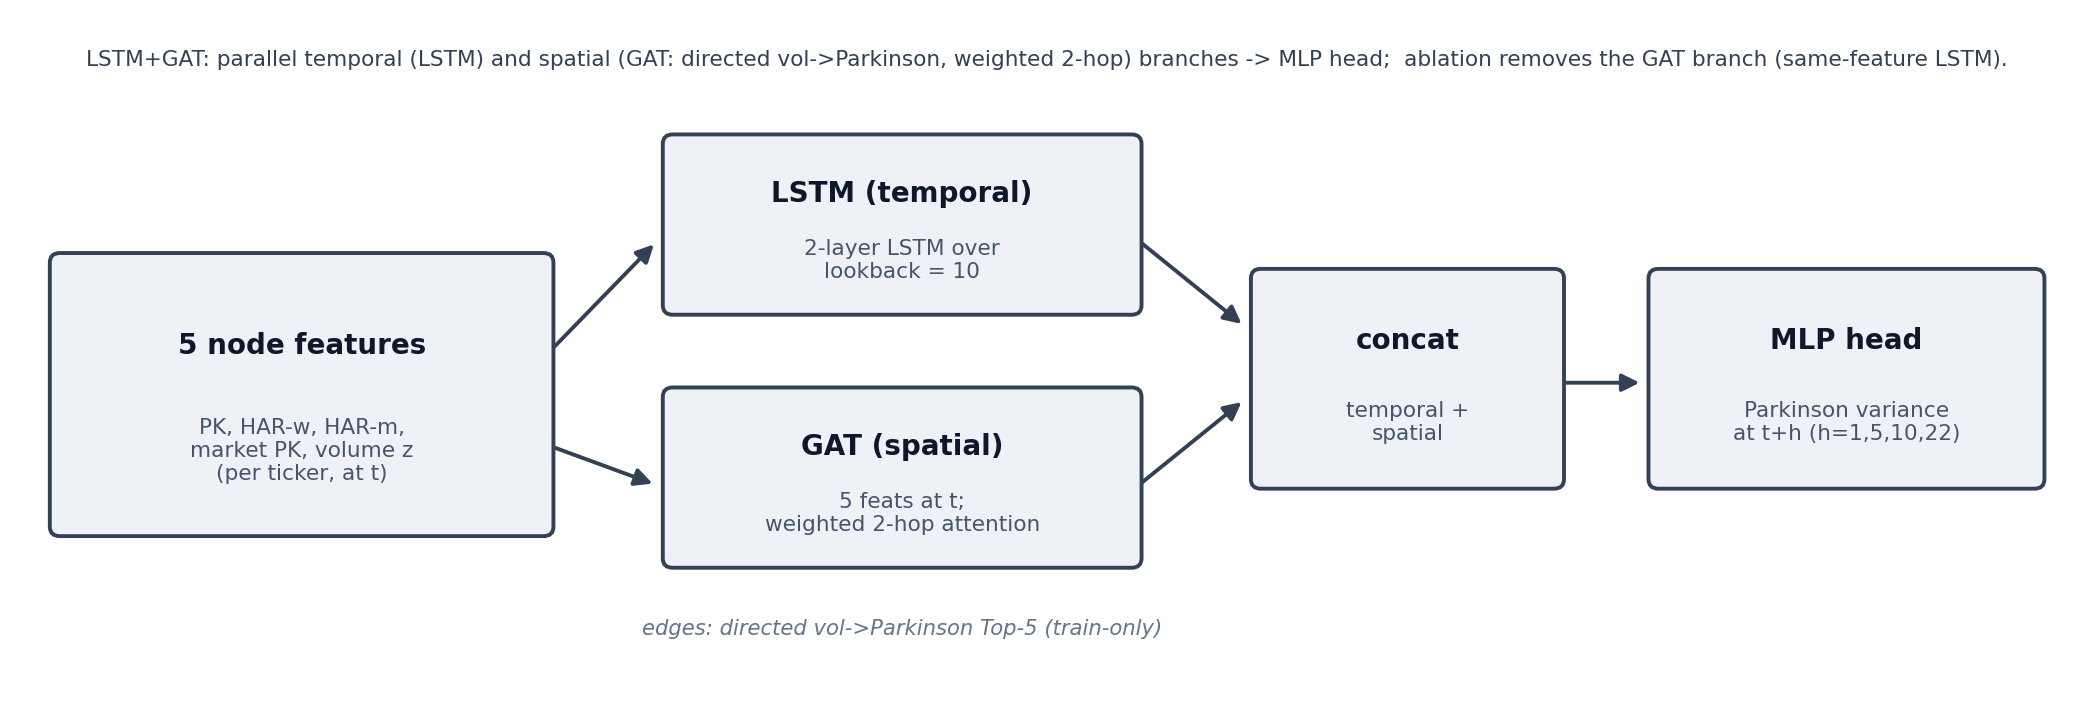
\includegraphics[width=\textwidth]{diagrams/soict_harlstmgat.png}
\caption{LSTM+GAT: a per-node LSTM temporal branch and a GAT spatial branch (directed volume$\to$Parkinson
Top-5 weighted two-hop attention) are concatenated into an MLP head; the leave-one-out comparison removes the
GAT branch to give the same-feature LSTM.}
\label{fig:arch}
\end{figure}

\section{Data}
Two panels are used with the Parkinson target: \textbf{VN30} (primary) and \textbf{VN100} (vnstock). Both use the masked panel of Sec.~3 with the five features, a single chronological
split and per-ticker standardization fit on training rows only.

\section{Experiments}
We compare HAR-X, the five-feature LSTM and the five-feature LSTM+GAT (directed volume$\to$Parkinson weighted
two-hop) on VN30 and VN100 over the masked panel at horizons $\{1,5,10,22\}$, reporting all
five metrics and the two targeted date-clustered DM contrasts (LSTM vs HAR-X, LSTM+GAT vs LSTM).

\section{Results}
Point-error metrics are scaled (MSE $\times10^{-7}$, RMSE $\times10^{-4}$, MAE $\times10^{-4}$); QLIKE and
$R^2$ unscaled. All values are five-seed test means (\texttt{results/masked\_rich\_floor1e2/}). Row order is
HAR-X $\to$ LSTM $\to$ LSTM+GAT. Tables~\ref{tab:vn100} and~\ref{tab:vn30} report all five metrics;
Table~\ref{tab:dm} reports the two targeted date-clustered DM contrasts on QLIKE and MAE. The primary horizons
$h1$/$h5$ appear first; the extended horizons $h10$/$h22$ appear in the lower block of each table.

\begin{table}[t]
\centering
\caption{VN100 (46{,}308 masked obs over 454 test dates at $h1$; 5-seed means). Lower is better
for MSE/RMSE/MAE/QLIKE, higher for $R^2$. $^{\dagger}$~marks metrics where LSTM+GAT improves over the no-graph LSTM. MSE $\times10^{-7}$, RMSE $\times10^{-4}$, MAE $\times10^{-4}$.}
\label{tab:vn100}
\footnotesize
\setlength{\tabcolsep}{5pt}
\begin{tabular}{llccccc}
\toprule
$h$ & Model & MSE & RMSE & MAE & QLIKE & $R^2$ \\
\midrule
1  & HAR-X     & 2.367 & 4.865 & 2.898 & 0.5115 & 0.2236 \\
1  & GARCH    & 3.816 & 6.178 & 4.538 & 0.7577 & -0.2519 \\
1  & LSTM     & 2.370 & 4.869 & 2.821 & 0.5525 & 0.2224 \\
1  & LSTM+GAT & \textbf{2.362}$^{\dagger}$ & \textbf{4.860}$^{\dagger}$ & \textbf{2.819}$^{\dagger}$ & \textbf{0.5107}$^{\dagger}$ & \textbf{0.2251}$^{\dagger}$ \\
\midrule
5  & HAR-X     & \textbf{2.606} & \textbf{5.104} & 3.160 & \textbf{0.5633} & \textbf{0.1466} \\
5  & GARCH    & 3.814 & 6.176 & 4.546 & 0.7420 & -0.2493 \\
5  & LSTM     & 2.638 & 5.136 & \textbf{3.090} & 0.5841 & 0.1361 \\
5  & LSTM+GAT & 2.635$^{\dagger}$ & 5.133$^{\dagger}$ & 3.103 & 0.5690$^{\dagger}$ & 0.1371$^{\dagger}$ \\
\midrule
\multicolumn{7}{l}{\emph{Extended horizons}}\\
10 & HAR-X     & \textbf{2.754} & \textbf{5.248} & 3.306 & \textbf{0.6023} & \textbf{0.0978} \\
10 & GARCH    & 3.891 & 6.238 & 4.582 & 0.7605 & -0.2745 \\
10 & LSTM     & 2.798 & 5.289 & 3.282 & 0.6070 & 0.0837 \\
10 & LSTM+GAT & 2.802 & 5.294 & \textbf{3.276}$^{\dagger}$ & 0.6072 & 0.0822 \\
\midrule
22 & HAR-X     & \textbf{2.891} & \textbf{5.377} & 3.486 & \textbf{0.6405} & \textbf{0.0544} \\
22 & GARCH    & 3.854 & 6.208 & 4.568 & 0.7450 & -0.2603 \\
22 & LSTM     & 2.979 & 5.458 & \textbf{3.468} & 0.6518 & 0.0257 \\
22 & LSTM+GAT & 3.003 & 5.480 & 3.563 & 0.6544 & 0.0178 \\
\bottomrule
\end{tabular}
\end{table}

\begin{table}[t]
\centering
\caption{VN30 (10{,}106 masked obs over 326 test dates at $h1$; 5-seed means). $^{\dagger}$~as in Table~1. Same scaling as
Table~\ref{tab:vn100}.}
\label{tab:vn30}
\footnotesize
\setlength{\tabcolsep}{5pt}
\begin{tabular}{llccccc}
\toprule
$h$ & Model & MSE & RMSE & MAE & QLIKE & $R^2$ \\
\midrule
1  & HAR-X     & 1.927 & 4.389 & 2.389 & \textbf{0.5159} & 0.2308 \\
1  & GARCH    & 2.788 & 5.280 & 3.480 & 0.7954 & -0.1129 \\
1  & LSTM     & 1.929 & 4.393 & 2.407 & 0.6073 & 0.2297 \\
1  & LSTM+GAT & \textbf{1.912}$^{\dagger}$ & \textbf{4.372}$^{\dagger}$ & \textbf{2.366}$^{\dagger}$ & 0.5800$^{\dagger}$ & \textbf{0.2368}$^{\dagger}$ \\
\midrule
5  & HAR-X     & \textbf{2.139} & \textbf{4.625} & \textbf{2.583} & \textbf{0.5965} & \textbf{0.1497} \\
5  & GARCH    & 2.783 & 5.276 & 3.489 & 0.7859 & -0.1065 \\
5  & LSTM     & 2.164 & 4.652 & 2.632 & 0.6402 & 0.1397 \\
5  & LSTM+GAT & 2.147$^{\dagger}$ & 4.633$^{\dagger}$ & 2.651 & 0.6059$^{\dagger}$ & 0.1467$^{\dagger}$ \\
\midrule
\multicolumn{7}{l}{\emph{Extended horizons}}\\
10 & HAR-X     & \textbf{2.301} & \textbf{4.797} & 2.733 & \textbf{0.6428} & \textbf{0.1028} \\
10 & GARCH    & 2.829 & 5.319 & 3.508 & 0.7774 & -0.1029 \\
10 & LSTM     & 2.310 & 4.806 & \textbf{2.721} & 0.6584 & 0.0995 \\
10 & LSTM+GAT & 2.326 & 4.823 & 2.725 & 0.6564$^{\dagger}$ & 0.0931 \\
\midrule
22 & HAR-X     & \textbf{2.272} & \textbf{4.766} & \textbf{2.785} & \textbf{0.6422} & \textbf{0.0723} \\
22 & GARCH    & 2.719 & 5.214 & 3.437 & 0.7452 & -0.1102 \\
22 & LSTM     & 2.383 & 4.881 & 2.904 & 0.6550 & 0.0271 \\
22 & LSTM+GAT & 2.385 & 4.883 & 2.884$^{\dagger}$ & 0.6548$^{\dagger}$ & 0.0261 \\
\bottomrule
\end{tabular}
\end{table}

\begin{table}[t]
\centering
\caption{Targeted date-clustered DM contrasts ($p$-value; favoured model in parentheses; bold if $p<0.05$).
H=HAR-X, L=LSTM, G=LSTM+GAT, on QLIKE and MAE.}
\label{tab:dm}
\footnotesize
\setlength{\tabcolsep}{5pt}
\begin{tabular}{ll cc cc}
\toprule
& & \multicolumn{2}{c}{LSTM vs HAR-X} & \multicolumn{2}{c}{LSTM+GAT vs LSTM} \\
\cmidrule(lr){3-4}\cmidrule(lr){5-6}
Panel & $h$ & QLIKE & MAE & QLIKE & MAE \\
\midrule
VN100 & 1  & \textbf{.028 (H)} & \textbf{$<$.001 (L)} & \textbf{$<$.001 (G)} & .684 (G) \\
VN100 & 5  & .148 (H) & \textbf{$<$.001 (L)} & \textbf{.022 (G)} & \textbf{.002 (L)} \\
VN100 & 10 & .598 (H) & .201 (L) & .872 (L) & .064 (G) \\
VN100 & 22 & .429 (H) & .611 (L) & .658 (L) & \textbf{$<$.001 (L)} \\
\midrule
VN30 & 1  & \textbf{$<$.001 (H)} & .221 (H) & \textbf{$<$.001 (G)} & \textbf{$<$.001 (G)} \\
VN30 & 5  & \textbf{.037 (H)} & \textbf{$<$.001 (H)} & \textbf{.031 (G)} & \textbf{.015 (L)} \\
VN30 & 10 & .260 (H) & .340 (L) & .547 (G) & .624 (L) \\
VN30 & 22 & .318 (H) & \textbf{.001 (H)} & .936 (G) & \textbf{.021 (G)} \\
\bottomrule
\end{tabular}
\end{table}

\textbf{Short-horizon results ($h1$, $h5$).} At VN100 $h1$ the LSTM+GAT has the lowest value on all five
metrics (MSE 2.362, RMSE 4.860, MAE 2.819, QLIKE 0.5107, $R^2$ 0.2251); by DM the LSTM has a lower MAE than HAR-X
($p<0.001$), a higher QLIKE than HAR-X ($p=0.028$), and the LSTM+GAT has a lower QLIKE than the no-graph LSTM
($p<0.001$). At VN100 $h5$ HAR-X has the lowest MSE, RMSE, QLIKE and highest $R^2$ and the LSTM the lowest MAE
(3.090); by DM the LSTM has a lower MAE than HAR-X ($p<0.001$) and the LSTM+GAT a lower QLIKE than the LSTM
($p=0.022$). At VN30 $h1$ the LSTM+GAT has the lowest MSE, RMSE, MAE and highest $R^2$ and HAR-X the lowest QLIKE
(0.5159); by DM the LSTM has a higher QLIKE than HAR-X ($p<0.001$) and the LSTM+GAT a lower QLIKE ($p<0.001$) and
squared error ($p=0.003$) than the no-graph LSTM. At VN30 $h5$ HAR-X has the lowest value on all five metrics; by
DM the LSTM has a higher QLIKE ($p=0.037$) and MAE ($p<0.001$) than HAR-X and the LSTM+GAT a lower QLIKE than the
LSTM ($p=0.031$). Across the four short-horizon cells no learned model has a significantly lower QLIKE than
HAR-X, and the LSTM+GAT has a significantly lower QLIKE than the no-graph LSTM in all four, equal to HAR-X's QLIKE
level at VN100 $h5$ (0.5690 vs 0.5633) and $h1$ (0.5107 vs 0.5115).

\textbf{Extended-horizon results ($h10$, $h22$).} HAR-X has the lowest MSE, RMSE, QLIKE and highest $R^2$ on both
panels at both horizons; the LSTM has the lowest MAE at VN100 $h22$ (3.468) and VN30 $h10$ (2.721), the
LSTM+GAT the lowest MAE at VN100 $h10$ (3.276). By DM the LSTM+GAT-vs-LSTM QLIKE difference is not significant
at $h10$ or $h22$ on either panel ($p\ge0.55$); the LSTM has a higher squared error than HAR-X at VN100 $h10$
($p=0.022$) and $h22$ ($p=0.002$) and a higher MAE than HAR-X at VN30 $h22$ ($p=0.001$).

\textbf{GARCH benchmark.} GARCH(1,1) has a higher MSE, RMSE, MAE and QLIKE and a lower $R^2$ than HAR-X at
every horizon on both panels, with a negative $R^2$ on both; its QLIKE is higher than HAR-X's under the
date-clustered DM test in all eight cells ($p<0.001$, except VN30 $h22$ where $p=0.001$). GARCH is a frozen-train forecast: a single conditional-variance path is projected from the end of training (persistence capped at 0.999 by variance targeting), so it cannot adapt to the level shifts that HAR-X re-estimates each day, and its error is correspondingly higher.

\textbf{Per-metric ranking.} No single metric determines the ordering, so all five are reported with equal
weight: HAR-X has the lowest QLIKE at every horizon except VN100 $h1$ (where the LSTM+GAT is marginally lower, not significantly), with no learned model significantly lower at any horizon; the deep and graph models have the lowest point error at the
short horizons; HAR-X has the lowest MSE/RMSE from $h5$ onward.

\section{Out-of-sample extension: broader Vietnamese universe (HOSE, HNX)}\label{sec:oos}
HOSE and HNX daily OHLCV were crawled and processed to the same Parkinson-variance target as VN30/VN100. A
liquidity-and-history screen (at least 250 rows per ticker and at most 50\% zero-variance days) was applied,
leaving the modelled universe reported by the \texttt{num\_nodes} field of each results file: 352 tickers on
HOSE and 154 on HNX (153 at $h22$). This universe was not used to design the model or to select any
configuration, so it is an untouched out-of-sample check. The same main configuration and protocol as
VN30/VN100 are used: the same five node features, the masked panel, the z-score$+$linear output with a
relative floor at $10^{-2}$ times the per-node training mean, five seeds and the date-clustered DM test. The
absolute QLIKE is higher than on VN30/VN100 because these panels are far less liquid; many low-range days
remain even after screening, which inflates the QLIKE level for every model.

\begin{table}[t]
\centering
\caption{HOSE (186{,}944 masked obs over 572 test dates at $h1$; 5-seed means). Lower is better for
MSE/RMSE/MAE/QLIKE, higher for $R^2$. $^{\dagger}$~marks metrics where LSTM+GAT improves over the no-graph
LSTM. MSE $\times10^{-7}$, RMSE $\times10^{-4}$, MAE $\times10^{-4}$.}
\label{tab:hose}
\footnotesize
\setlength{\tabcolsep}{5pt}
\begin{tabular}{llccccc}
\toprule
$h$ & Model & MSE & RMSE & MAE & QLIKE & $R^2$ \\
\midrule
1  & HAR-X    & 3.299 & 5.744 & 3.309 & \textbf{1.2342} & 0.1854 \\
1  & GARCH    & 18.495 & 13.600 & 5.878 & 1.4865 & -3.5660 \\
1  & LSTM     & \textbf{3.269} & \textbf{5.717} & \textbf{3.219} & 1.2443 & \textbf{0.1931} \\
1  & LSTM+GAT & 3.273 & 5.721 & 3.232 & 1.2432$^{\dagger}$ & 0.1921 \\
\midrule
5  & HAR-X    & \textbf{3.610} & \textbf{6.009} & 3.647 & \textbf{1.2963} & \textbf{0.1091} \\
5  & GARCH    & 6.151 & 7.843 & 5.223 & 1.4767 & -0.5179 \\
5  & LSTM     & 3.627 & 6.022 & \textbf{3.574} & 1.3137 & 0.1051 \\
5  & LSTM+GAT & 3.646 & 6.038 & 3.680 & 1.3025$^{\dagger}$ & 0.1002 \\
\midrule
\multicolumn{7}{l}{\emph{Extended horizons}}\\
10 & HAR-X    & \textbf{3.744} & \textbf{6.118} & \textbf{3.807} & 1.3387 & \textbf{0.0774} \\
10 & GARCH    & 5.503 & 7.418 & 5.125 & 1.4871 & -0.3563 \\
10 & LSTM     & 3.820 & 6.180 & 3.895 & 1.3367 & 0.0586 \\
10 & LSTM+GAT & 3.801$^{\dagger}$ & 6.165$^{\dagger}$ & 3.871$^{\dagger}$ & \textbf{1.3348}$^{\dagger}$ & 0.0633$^{\dagger}$ \\
\midrule
22 & HAR-X    & \textbf{3.878} & \textbf{6.227} & \textbf{3.995} & 1.3820 & \textbf{0.0449} \\
22 & GARCH    & 5.592 & 7.478 & 5.141 & 1.4880 & -0.3773 \\
22 & LSTM     & 3.981 & 6.309 & 4.068 & \textbf{1.3774} & 0.0195 \\
22 & LSTM+GAT & 3.998 & 6.323 & 4.119 & 1.3803 & 0.0152 \\
\bottomrule
\end{tabular}
\end{table}

\begin{table}[t]
\centering
\caption{HNX (62{,}004 masked obs over 489 test dates at $h1$; 5-seed means). $^{\dagger}$~as in
Table~\ref{tab:hose}. Same scaling as Table~\ref{tab:hose}.}
\label{tab:hnx}
\footnotesize
\setlength{\tabcolsep}{5pt}
\begin{tabular}{llccccc}
\toprule
$h$ & Model & MSE & RMSE & MAE & QLIKE & $R^2$ \\
\midrule
1  & HAR-X    & 13.986 & 11.826 & 6.549 & 1.8717 & 0.2154 \\
1  & GARCH    & 21.336 & 14.607 & 9.503 & 2.1065 & -0.1969 \\
1  & LSTM     & 13.717 & 11.712 & 6.438 & \textbf{1.8128} & 0.2305 \\
1  & LSTM+GAT & \textbf{13.706}$^{\dagger}$ & \textbf{11.707}$^{\dagger}$ & \textbf{6.415}$^{\dagger}$ & 1.8135 & \textbf{0.2312}$^{\dagger}$ \\
\midrule
5  & HAR-X    & 15.495 & 12.448 & 7.123 & 1.9402 & 0.1273 \\
5  & GARCH    & 19.960 & 14.128 & 9.268 & 2.1052 & -0.1241 \\
5  & LSTM     & \textbf{15.423} & \textbf{12.419} & \textbf{7.103} & \textbf{1.9318} & \textbf{0.1314} \\
5  & LSTM+GAT & 15.465 & 12.436 & 7.193 & 1.9356 & 0.1290 \\
\midrule
\multicolumn{7}{l}{\emph{Extended horizons}}\\
10 & HAR-X    & 15.977 & 12.640 & \textbf{7.361} & 1.9904 & 0.0970 \\
10 & GARCH    & 19.832 & 14.083 & 9.301 & 2.2020 & -0.1209 \\
10 & LSTM     & 16.004 & 12.651 & 7.482 & 1.9830 & 0.0955 \\
10 & LSTM+GAT & \textbf{15.975}$^{\dagger}$ & \textbf{12.639}$^{\dagger}$ & 7.450$^{\dagger}$ & \textbf{1.9815}$^{\dagger}$ & \textbf{0.0971}$^{\dagger}$ \\
\midrule
22 & HAR-X    & \textbf{16.554} & \textbf{12.866} & \textbf{7.635} & 2.0391 & \textbf{0.0681} \\
22 & GARCH    & 18.948 & 13.765 & 9.107 & 2.1254 & -0.0667 \\
22 & LSTM     & 16.665 & 12.909 & 7.869 & 2.0315 & 0.0619 \\
22 & LSTM+GAT & 16.591$^{\dagger}$ & 12.880$^{\dagger}$ & 7.767$^{\dagger}$ & \textbf{2.0281}$^{\dagger}$ & 0.0661$^{\dagger}$ \\
\bottomrule
\end{tabular}
\end{table}

\begin{table}[t]
\centering
\caption{Out-of-sample date-clustered DM contrasts on HOSE and HNX ($p$-value; favoured model in
parentheses; bold if $p<0.05$). H=HAR-X, L=LSTM, G=LSTM+GAT, on QLIKE and MAE.}
\label{tab:dmext}
\footnotesize
\setlength{\tabcolsep}{4pt}
\begin{tabular}{ll cc cc cc}
\toprule
& & \multicolumn{2}{c}{LSTM vs HAR-X} & \multicolumn{2}{c}{LSTM+GAT vs HAR-X} & \multicolumn{2}{c}{LSTM+GAT vs LSTM} \\
\cmidrule(lr){3-4}\cmidrule(lr){5-6}\cmidrule(lr){7-8}
Panel & $h$ & QLIKE & MAE & QLIKE & MAE & QLIKE & MAE \\
\midrule
HOSE & 1  & .553 (H) & \textbf{$<$.001 (L)} & .593 (H) & \textbf{$<$.001 (G)} & .649 (G) & \textbf{$<$.001 (L)} \\
HOSE & 5  & .163 (H) & \textbf{$<$.001 (L)} & .384 (H) & \textbf{.005 (H)} & .095 (G) & \textbf{$<$.001 (L)} \\
HOSE & 10 & .674 (L) & \textbf{$<$.001 (H)} & .343 (G) & \textbf{$<$.001 (H)} & .108 (G) & \textbf{$<$.001 (G)} \\
HOSE & 22 & .442 (L) & \textbf{.020 (H)} & .712 (G) & \textbf{$<$.001 (H)} & .080 (L) & \textbf{$<$.001 (L)} \\
\midrule
HNX & 1  & \textbf{$<$.001 (L)} & \textbf{$<$.001 (L)} & \textbf{$<$.001 (G)} & \textbf{$<$.001 (G)} & .560 (L) & \textbf{$<$.001 (G)} \\
HNX & 5  & \textbf{.050 (L)} & .404 (L) & .178 (G) & \textbf{$<$.001 (H)} & \textbf{.023 (L)} & \textbf{$<$.001 (L)} \\
HNX & 10 & .065 (L) & \textbf{$<$.001 (H)} & \textbf{.022 (G)} & \textbf{$<$.001 (H)} & \textbf{.015 (G)} & \textbf{$<$.001 (G)} \\
HNX & 22 & .094 (L) & \textbf{$<$.001 (H)} & \textbf{.016 (G)} & \textbf{$<$.001 (H)} & \textbf{.031 (G)} & \textbf{$<$.001 (G)} \\
\bottomrule
\end{tabular}
\end{table}

\textbf{Interpretation.} On HNX the deep models attain a significantly lower QLIKE than HAR-X at $h1$
(LSTM and LSTM+GAT, $p<0.001$), $h10$ (LSTM+GAT, $p=0.022$) and $h22$ (LSTM+GAT, $p=0.016$), with the LSTM
borderline at $h5$ ($p=0.050$); the LSTM+GAT also has a significantly lower QLIKE than the no-graph LSTM at
$h10$ ($p=0.015$) and $h22$ ($p=0.031$). The temporal and graph value that is absent on the liquid VN30/VN100
blue chips thus appears on the broader, less-liquid HNX universe. On HOSE no learned model differs
significantly from HAR-X on QLIKE at any horizon ($p\ge0.16$); the deep models still have the lowest MAE at
$h1$ ($p<0.001$), which reverses at $h10$/$h22$ where HAR-X has the lower MAE ($p<0.001$--$0.020$). GARCH is
far worse on both exchanges, with a negative $R^2$ (down to $-3.6$ on HOSE $h1$) and a significantly
higher QLIKE than HAR-X in every cell ($p<0.001$), consistent with a single frozen-train conditional-variance
path that cannot track the panels' level shifts.
These are out-of-sample observations from a single configuration on one holdout; they motivate, but do not by
themselves establish, the deep and graph advantage on less-liquid Vietnamese equities.

\section{Discussion}\label{sec:disc}
No learned model has a significantly lower QLIKE than HAR-X at any horizon under the date-clustered DM test;
HAR-X has the lowest point estimate in every cell except VN100 $h1$, where the LSTM+GAT is marginally lower
(not significant). At $h1$ and $h5$ the LSTM and LSTM+GAT have the lowest MAE on VN100
(LSTM vs HAR-X, $p<0.001$), and the LSTM+GAT has a significantly lower QLIKE and, on VN30, lower squared error
than the same-feature no-graph LSTM; at VN100 $h1$ and VN30 $h1$ the LSTM+GAT has the lowest value on four or
five of the metrics. At $h10$ and $h22$ HAR-X has the lowest MSE, RMSE, QLIKE and $R^2$, and the
LSTM+GAT-vs-LSTM QLIKE difference is not significant. The graph's effect on QLIKE relative to the no-graph LSTM
is present at the short horizons and absent at the longer horizons; the deep models' MAE reduction is present
at the short horizons on VN100 and reverses at the longer horizons, where their squared error and MAE are
higher than HAR-X's. The ranking is metric- and horizon-dependent, which is why all five metrics are reported
with equal weight. The date-clustered DM test matters for these conclusions: a naive per-observation test on
this cross-sectionally dependent panel inflates the statistic by roughly the square root of the number of stocks, so a difference
that is not significant per date can appear significant per observation.

\section{Conclusion}
For daily Parkinson-variance forecasting on the Vietnamese market, evaluated with the same features, the same
masked panel and the same date-clustered Diebold--Mariano inference, no learned model has a significantly lower
QLIKE than HAR-X at any horizon, and HAR-X has the lowest QLIKE point estimate in every cell except VN100 $h1$,
where the LSTM+GAT is marginally lower (not significant). At the short
horizons ($h1$, $h5$) the LSTM and LSTM+GAT have the lowest MAE on VN100, and the directed volume$\to$Parkinson
weighted graph gives the LSTM+GAT a significantly lower QLIKE than the same-feature no-graph LSTM in both
panels, equal to HAR-X's QLIKE level at VN100 $h5$; at the extended horizons ($h10$, $h22$) HAR-X has the lowest
MSE, RMSE, QLIKE and $R^2$, and the graph's QLIKE difference from the no-graph LSTM is not significant. The
ranking is metric- and horizon-dependent, so all five metrics are reported with equal weight.

\begin{thebibliography}{99}
\bibitem{corsi2009} Corsi, F.: A simple approximate long-memory model of realized volatility. J. Financial Econometrics \textbf{7}(2), 174--196 (2009)
\bibitem{parkinson1980} Parkinson, M.: The extreme value method for estimating the variance of the rate of return. J. Business \textbf{53}(1), 61--65 (1980)
\bibitem{lstm1997} Hochreiter, S., Schmidhuber, J.: Long short-term memory. Neural Computation \textbf{9}(8), 1735--1780 (1997)
\bibitem{gat2018} Veli\v{c}kovi\'c, P., et al.: Graph attention networks. In: ICLR (2018)
\bibitem{dm1995} Diebold, F.X., Mariano, R.S.: Comparing predictive accuracy. J. Business \& Economic Statistics \textbf{13}(3), 253--263 (1995)
\bibitem{hln1997} Harvey, D., Leybourne, S., Newbold, P.: Testing the equality of prediction mean squared errors. Int. J. Forecasting \textbf{13}(2), 281--291 (1997)
\bibitem{patton2011} Patton, A.J.: Volatility forecast comparison using imperfect volatility proxies. J. Econometrics \textbf{160}(1), 246--256 (2011)
\bibitem{harq2016} Bollerslev, T., Patton, A.J., Quaedvlieg, R.: Exploiting the errors: a simple approach for improved volatility forecasting. J. Econometrics \textbf{192}(1), 1--18 (2016)
\bibitem{chen2022} Chen, Q., Robert, C.-Y.: Multivariate realized volatility forecasting with graph neural network. In: ACM ICAIF (2022). arXiv:2112.09015
\bibitem{gnnhar2025} Zhang, C., Pu, X., Cucuringu, M., Dong, X.: Forecasting realized volatility with spillover effects: perspectives from graph neural networks (2025). arXiv:2308.01419
\bibitem{dy2012} Diebold, F.X., Yilmaz, K.: Better to give than to receive: predictive directional measurement of volatility spillovers. Int. J. Forecasting \textbf{28}(1), 57--66 (2012)
\bibitem{audrino2025} Audrino, F., Chassot, J.: HARd to beat: the overlooked impact of rolling windows in the era of machine learning. Int. J. Forecasting (2025). arXiv:2406.08041
\end{thebibliography}

\end{document}
